\section{Unfolding of CPNs}

The extensions of Petri nets that CPNs bring in the form of a
programming language and modules add practical modelling power to
Petri nets by making it easier to construct models of complex
systems. The extensions do not add expressive power from a theoretical
perspective as any hierarhical CPN model can be unfolded to a
non-hierarhical CPN model which in turn can be unfolded to a
behaviorally equivalence and possibly infinite Place Transition
Net. Furthermore, each Place Transition Net can be folded into a CPN
with a single module consisting of a single place and a single
transition. In practice such a folding is totally uninteresting,
because the arc expressions will be extremely complex and totally
non-interpretable for a human being. However, the fact that the
unfolding and folding exists shows that hierarchical CPNs has the same
theoretical properties as basic Petri nets - in particular that CPNs
are a solid model for concurrency, conflict synchronization and
resource sharing. The unfolding of a hierarhical CPN model to a
non-hierarhical consists of recursively replacing each substitution
transition with its associated submodule such that related port and
socket places are merge into a single place. The unfolding of a
non-hierarchical CPN model to an ordinary Petri net consists of
unfolding each high-level places to a place for color in the color set
of the high-level place, and unfolding each transition to a transition
for each possible binding of the high-level transition.

%Anything which can be programming in Java can (in theory) also be
%programmed in assembler code. It is just much more time-consuming and
%much more error-prone. 

%Analogously it can be proved (quite easily) that each hierarchical CPN
%can be unfolded to a (much larger) basic Petri net (Place Transition
%Net) with exactly the same dynamic behavior.

% illustrate place unfolding

To illustrate the unfolding high-level place consider the CPN model
fragment shown in Fig.~\ref{fig:sendcancommit}. To represent this
fragment as an ordinary Petri net, place \figitem{CanCommit} needs to
be unfolding to a place corresponding to \smlcode{wrk(1)} and
\smlcode{wrk(2)}. The place \figitem{Idle} and \figitem{WaitingVotes}
does not need to be unfolding as the \smlcode{Unit} color set contains
just a single value. Similarly, no unfolding of the
\figitem{SendCanCommit} transition is required in this case since the
transition does not have any variables. The equivalent Place
Transition Net is shown in Fig,~\ref{fig:sendcancommitunfold}. It can
be seen that the arc expression are replace by arc weights and the
initial marking is replace by the specification of a single token
initially in \figitem{Idle}.

\begin{figure}[h]
\centering
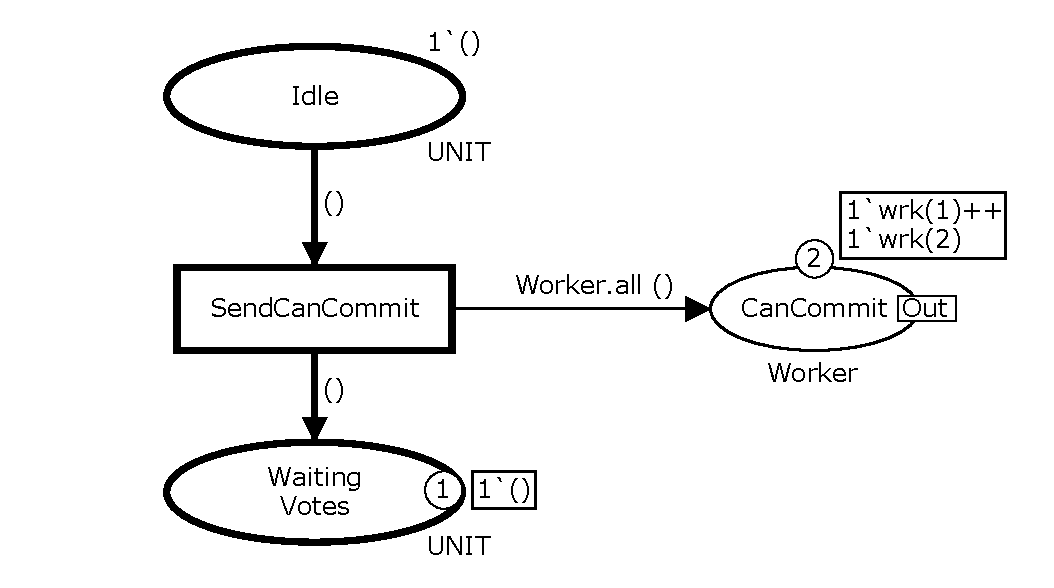
\includegraphics[scale=.5]{figures/SendCanCommit.eps}
\caption{Current marking after \figitem{SendCanCommit}.}
\label{fig:sendcancommit}
\end{figure}

% illustrate transition unfolding

To illustrate the unfolding of a high-level transition consider the
CPN model fragment shown in Fig.~\ref{fig:receivecancommit}. To
represent this as a Place/Transition Net we need to unfold the place
as explained in the previous paragraph and in addition unfold the
transition \figitem{fig:receivecancommit} to a low-level transition
corresponding to each of the four binding elements listed in
Fig.~\ref{fig:XX}. Figure~\ref{fig:receivecancommitunfold} shows the
corresponding Place Transition Net fragment. It can be seen that we
essentially need a copy of the CPN fragment for each worker in the
system.

\begin{figure}[h]
\centering
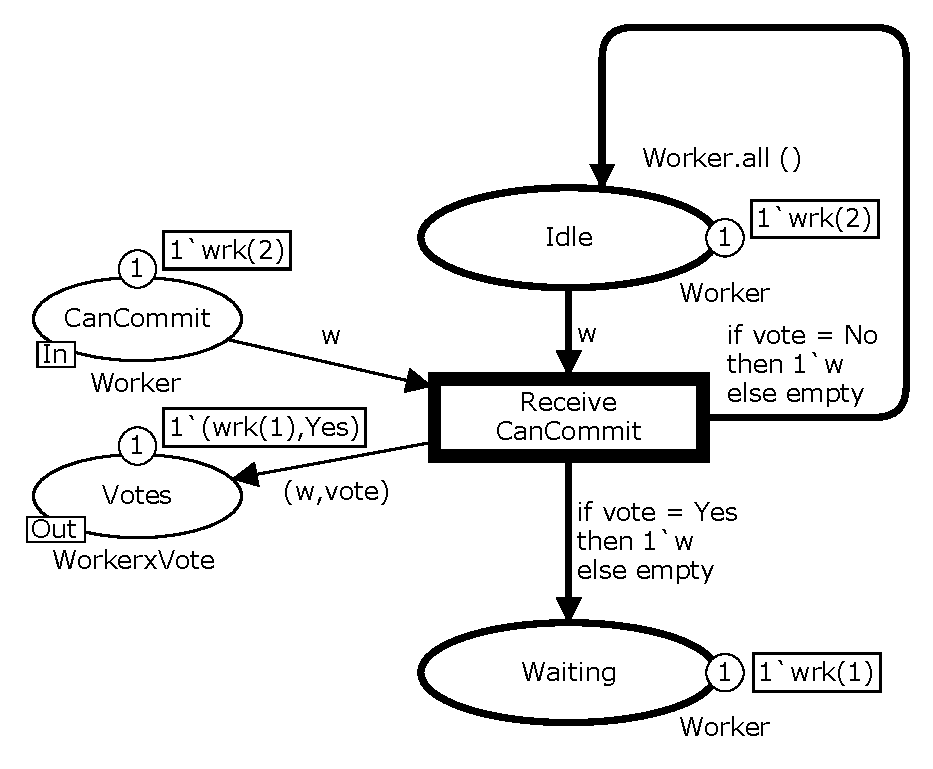
\includegraphics[scale=.5]{figures/ReceiveCanCommit.eps}
\caption{Current marking after \figitem{ReceiveCanCommit}.}
\label{fig:receivecancommit}
\end{figure}

The unfolding of the fragments above also illustrates that Petri nets
do not provide a way to easily scale the model according to some
system parameter (in this case the number of workers). With ordinary
Petri nets is is necessary to have a subnet for each worker (even
though they behave in exactly the same way). With PrT nets and CPNs we
can use tokens with color \smlcode{wrk(1)} to model the state of the
first worker, tokens with the color \smlcode{wrk(2)} to model the
state of the second worker, and so on. This means that we for
\smlcode{W} workers can have a single \figitem{Idle} place, which may
contain tokens of \smlcode{W} different colors - instead of having a
separate \smlcode{Idle} place for each of the \smlcode{W} workers. In
particular, in the CPN model where we just need to change the symbolic
constant \smlcode{W} (see Fig.~\ref{fig:coloursets}) to configure the
model to handle, e.g., five workers whereas with basic Petri nets we
need to add place, transitions, and arcs and hence change the net
structure in order to increase the number of workers.  This shows that
CPNs provides a means for easily creating parameterizable models and
also that it enables more compact modeling as we only need a single
instance of the \figitem{CanCommit} place in order to accommodate any
finite number of workers. Comparing CPN and PrT nets. With CPN it is
possible to have many color sets and hence we can use a number of
different color sets (e.g. one color set for the coordinator, a second
for the workers, a third for Yes/no votes and a fourth for
abort/commit decisions). With PrT nets only one set of token colors
are allowed (or cartesian product thereof) and hence with PrT nets we
could have had to represent the identity workers, Yes/No votes and
abort/commit decisions by colors based on this single set of token
colors.
